\documentclass[11pt]{article}
\usepackage{fullpage}
\usepackage{graphicx}
\usepackage{amssymb}
\usepackage{epstopdf}
\usepackage{amsmath}
\usepackage{float}
\usepackage{caption}
\DeclareGraphicsRule{.tif}{png}{.png}{`convert #1 `dirname #1`/`basename #1 .tif`.png}
\def\mathbi#1{\textbf{\em #1}}

%% LyX 1.4.1 created this file.  For more info, see http://www.lyx.org/.
%% Do not edit unless you really know what you are doing.
%\documentclass[11pt,english]{article}
%\usepackage{ae}
%\usepackage{aecompl}
%\usepackage[T1]{fontenc}
%\usepackage{geometry}
%\geometry{verbose,letterpaper,tmargin=1.25in,bmargin=1.25in,lmargin=1.25in,rmargin=1.25in}
%\pagestyle{empty}
%\usepackage{amsmath}
%\documentclass [11pt]{article}
\usepackage{graphicx}
%\pagestyle{myheadings}

\textheight 8.5in
\oddsidemargin 0.25in
\evensidemargin 0.25in
\textwidth 6.0in
\topmargin 0.25in
\headsep 0pt
\headheight 0pt


%\usepackage{setspace}
%\doublespacing
%\usepackage{amssymb}
%\usepackage[authoryear]{natbib}
%\usepackage{url}
%\usepackage{wrapfig}
%\usepackage{overcite}
%\usepackage{nsf}
%\usepackage{times}

\def\pmb#1{\setbox0=\hbox{#1}%
  \kern-.025em\copy0\kern-\wd0 
  \kern.05em\copy0\kern-\wd0
  \kern-.025em\raise.0433em\box0 } 
\def\picture #1 by #2 (#3){
  \vbox to #2{
   \hrule width #1 height 0pt depth 0pt
   \vfill
   \special{picture #3}}}
\def\scaledpicture #1 by #2 (#3 scaled #4){{
  \dimen0=#1 \dimen1=#2
  \divide\dimen0 by 1000 \multiply\dimen0 by #4
  \divide\dimen1 by 1000 \multiply\dimen1 by #4
  \picture \dimen0 by \dimen1 (#3 scaled #4)}}
\def\reff{\par\noindent\hangindent=10pt\hangafter=1}
\def\refff{\par\hangindent=30pt\hangafter=1}
%\newcommand{\te}[1]{\mbox{\boldmath$ #1 $}} 
%\newcommand{\te}[1]{\mbox{\bf $#1$ }}
\def\ba{\te{a}}
\def\bx{\te{x}}
\def\by{\te{y}}
\def\bz{\te{z}}
\def\bq{\te{q}}
\def\bu{\te{u}}
\def\bm{\te{m}}
\def\bI{\te{I}}
\def\bU{\te{U}}
\def\bX{\te{X}}
\def\bk{\te{k}}
\def\bB{\te{B}}
\def\bj{\te{j}}
\def\bD{\te{D}}
\def\bM{\te{M}}
\def\br{\te{r}}
\def\bb{\te{b}}
\def\bd{\te{d}}
\def\bR{\te{R}}
\def\bV{\te{V}}
\def\bS{\te{S}}
\def\bF{\te{F}}
\def\bE{\te{E}}
\def\bt{\te{t}}
\def\bn{\te{n}}
\def\bL{\te{L}}
\def\bg{\te{g}}
\def\bv{\te{v}}
\def\b1{\te{1}}
\def\bT{\te{T}}
% \def\mathbi#1{\textbf{\em #1}}
\newcommand{\mcd}{\mathcal{D}}


\newcommand{\te}[1]{\mbox{\boldmath$ #1 $}}

\usepackage{wrapfig}

\title{\emph{fmc}: efficient flow map calculation and its application to FTLE fields}
\author{D. M. Luchtenburg and B. J. Landrum}

\begin{document}
\maketitle

\begin{figure}[H]
\centering
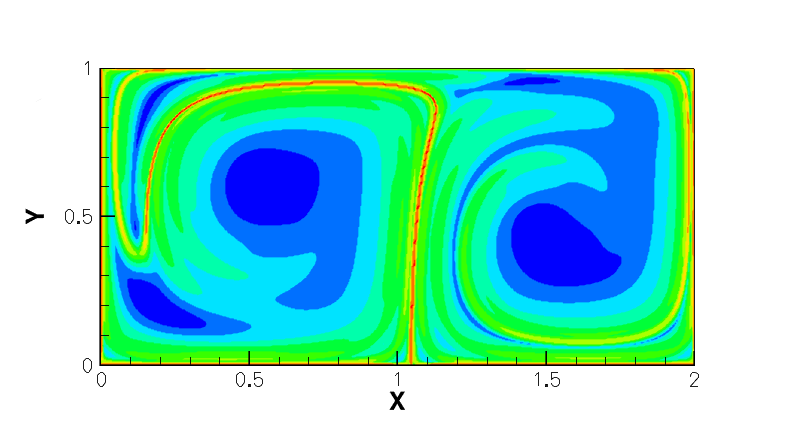
\includegraphics[scale=0.4]{images/ftle_gyre.png}
\caption*{Sample output: FTLE field computed for the double gyre}
\end{figure}

\tableofcontents

\section{Introduction}\label{toc:intro}

We develop a C++ software package that calculates the Finite-Time Lyapunov Exponent (FTLE) field of a 2D velocity field. Computation of the FTLE field requires calculation of the flow map associated with the velocity field. The flow map is efficiently computed in two steps. In the first step, short-time flow maps are approximated by a spectral basis, and in the second step, flow map composition is used to construct the long-time flow map. 

\subsection{Flow map and FTLE field}
Consider a dynamical system, which provides a 2D velocity field,  on a domain $\mcd\subseteq \mathbb{R}^2$:
\begin{equation}\label{dynamics}
    \dot x = f(x,t)
\end{equation}
where $x\in \mcd$ and $f:\mcd\times \mathbb{R}\rightarrow \mathbb{R}^2$ is Lipschitz continuous.  Given an initial condition
\begin{align}\label{initialcondition}
    x(t_0) = x_0, 
\end{align}
we denote trajectories by $x(t; t_0,x_0)$.

The \emph{flow map} $\phi_{t_0}^{t_f}:\mcd\rightarrow \mcd$ maps \emph{all} $x_0 \in \mcd$ to $x(t_f;t_0,x_0)$ and is given by:
    \begin{align}\label{flowmap}
        \phi_{t_0}^{t_f}:x(t_0)&\mapsto x(t_0)+\int_{t_0}^{t_f}f(x(\tau),\tau)d\tau
    \end{align}
The corresponding Jacobian matrix is given by:
\begin{align}\label{jacobian}
    J_{t_0}^{t_f}(x) = D_x \, \phi_{t_0}^{t_f}(x),
\end{align}
where $D_x$ denotes differentiation with respect to $x$. The \emph{Finite-Time Lyapunov Exponent} can now be defined as:
\begin{align}\label{ftle}
    \mu_{t_0}^{t_f}(x) = \frac{1}{t_f - t_0} \ln\left(\sigma\left(J_{t_0}^{t_f}(x)\right)\right),
\end{align}
where $\sigma$ denotes the maximum singular value of the Jacobian matrix. The FTLE is a scalar value which characterizes the amount of stretching about the trajectory of a traveling particle over the time interval $ [t_0, t_f]$.

\begin{flushleft}\textbf{Remark} We note that the velocity field $f(x,t)$, i.e.~the right-hand side of \eqref{dynamics}, can be provided 1) analytically, or 2) in the form of snapshots (velocity data at discrete spatial points at discrete instances in time). Our software supports both possibilities.
\end{flushleft}

\subsection{Flow map approximation and composition}
Consider the flow map \eqref{flowmap}. Let $t_0=\tau$ and $t_f=\tau + \Delta t$, where $\Delta t$ is ``small''. Then, we approximate the short-time flow map $\phi_{\tau}^{\tau+\Delta t}(x)$ by the expansion:
\begin{align}\label{flowmap_app}
    \phi_{\tau}^{\tau + \Delta t}(x_1,x_2) \approx \sum_{i=0}^{N_1} \sum_{j=0}^{N_2} \hat{\phi}_{ij} \, \Gamma_i(x_1) \Gamma_j(x_2), 
\end{align}
where the basis functions are (known) Legendre polynomials. The coefficients $\hat{\phi}_{ij}$ are computed using a so-called discrete Galerkin projection\footnote{Note that $x_1$, $x_2$ are defined on the standard element $[-1,1] \times [-1,1]$. For other domains, one can employ a linear transformation to scale to the standard element.}
\begin{align}\label{dgp}
    \hat{\phi}_{ij} & = \frac{1}{\gamma_i \gamma_j} \int_{-1}^1 \int_{-1}^1 \phi_{\tau}^{\tau +\Delta t}(x,y) \Gamma_i(x_1) \Gamma_j(x_2) dx dy \nonumber\\ 
    & \approx  \frac{1}{\gamma_i \gamma_j} \sum_{m=0}^{Q_1} \sum_{n=0}^{Q_2} \phi_{\tau}^{\tau + \Delta t}(x_1^{(m)},x_2^{(n)}) \Gamma_i(x_1^{(m)}) \Gamma_j(x_2^{(n)}) w^{(m)} w^{(n)},
\end{align}
where $\gamma_i$ is a normalization factor, $w^{(i)}$ a suitable quadrature weight, and $Q_i$ is the number of quadrature points. We use the Gauss-Lobatto points, and set $Q_i=N_i$. Thus, we need to compute the short time flow map at the quadrature points, i.e.~$\phi_{\tau}^{\tau + \Delta t}(x_1^{(m)},x_2^{(n)})$ for $m=0,\ldots,N_1$, $n=0,\ldots,N_2$.

We use \emph{flow map composition} to compute long-time flow maps $\phi_{t_0}^{t_0+T}$, where $T$ is ``large''. For $t_0=0$, $T=N\Delta t$, and equally spaced intermediate short-time maps with duration $\Delta t$, this becomes:
\begin{align}\label{flowmapcomp}
    \phi_{0}^{N\Delta t}=\phi_{(N-1)\Delta t}^{N\Delta t}\circ \cdots \circ \phi_{\Delta t}^{2\Delta t}\circ\phi_0^{\Delta t}.
\end{align}

\subsection{Program flow}

\begin{figure}[h]
\centering
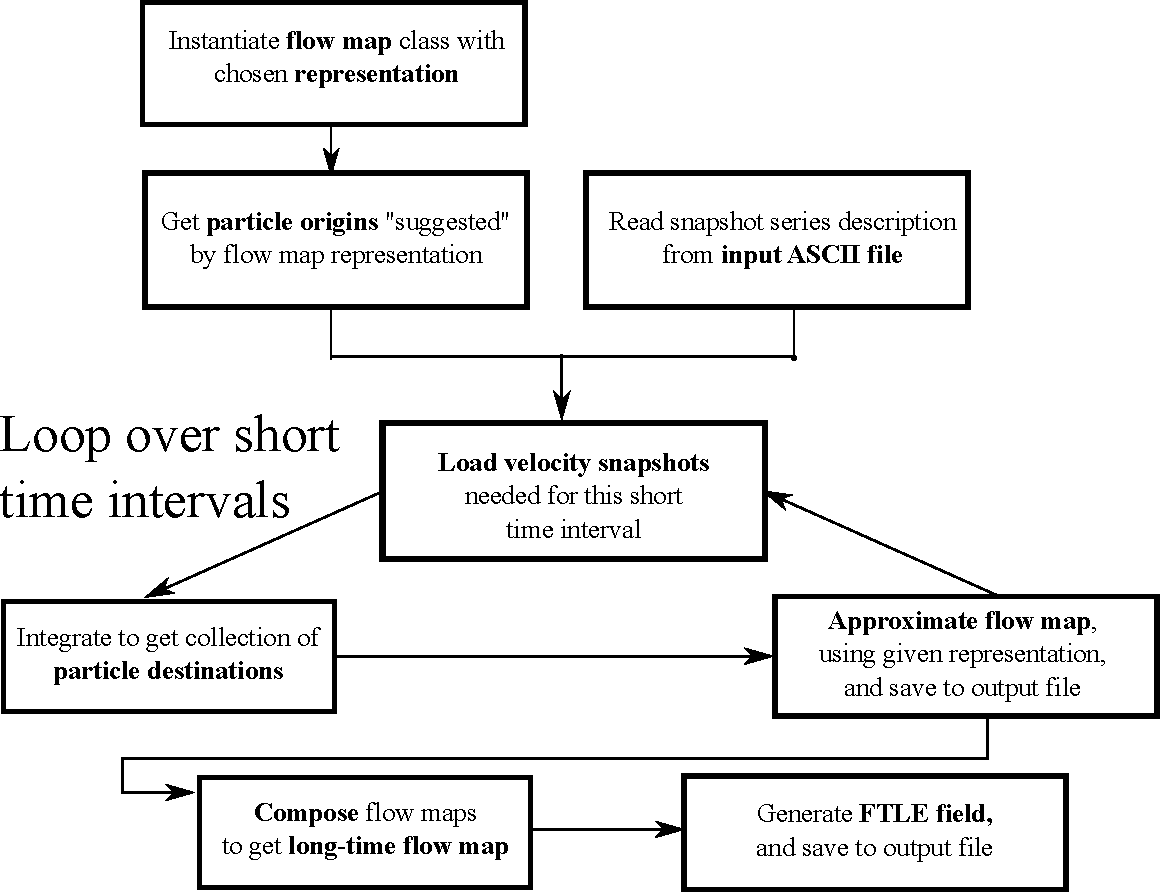
\includegraphics[scale=0.5]{images/program_flow.pdf}
\end{figure}

In summary, our program involves the following steps:
\begin{enumerate}
    \item The approximation of $N$ short time flow maps, see \eqref{flowmap_app}, for a time span $[0, N \Delta t]$. Employing \eqref{dgp}, this requires solution of \eqref{dynamics} where the initial conditions \eqref{initialcondition} are the quadrature points. 
    \item Composition of the short time flow maps to obtain the long-time flow map at $t=T$, see \eqref{flowmap}.
    \item Computation of the FTLE field at time $t=T$ using the flow map representation. Using \eqref{flowmap_app} and \eqref{flowmapcomp}, an analytical representation for the Jacobian \eqref{jacobian} can be derived. For simplicity, we consider finite difference approximations. The FLTE field is then calculated using \eqref{ftle}.
\end{enumerate}


\section{Installation}
Building \emph{fmc} from source requires a C++ compiler (we use \emph{g++}).  To install \emph{fmc} on a Linux system, simply {\tt cd} to the main directory and type {\tt make}.  This will compile two main programs: {\tt fmc-gyre} and {\tt fmc-snaps}, as well as a test suite, which runs automatically.  It is possible to make any one of these targets separately, using {\tt make fmc-gyre} or {\tt make fmc-snaps} or {\tt make test}.  {\tt make clean} removes the object files linked to build the executables.  {\tt fmc-gyre} and {\tt fmc-snaps} will be in the {\tt build} directory.

Changing settings for the compilation process -- setting the compiler, allowing for debugging, enabling warnings -- can be done by editing the {\tt make.inc} file in the config directory.

\section{User interface and how to run}

\subsection{Command-line input}
The user has two options:
\begin{enumerate}
    \item To compute the FTLE field of an analytically defined double-gyre velocity field, simply type\\
    {\tt fmc-gyre <integrator> <timestep> <numsteps> <order> <mgrid> <ngrid>},\\
    where integrator is the timestepper (Heun, or RungeKutta4). In the notation of Section \ref{toc:intro}, timestep is $\Delta t$, numsteps is $N$, order is $N_1 + N_2$ (the maximum order of the short-time flow map expansion). The last two options mgrid, ngrid specify the dimension of the grid for vizualisation in x- and y-direction.

    \item To run generate the same output using gridded velocity snapshots as input, you must type the following (quantities in brackets are command-line options described below):

\begin{verbatim}
fmc-snaps [snap_list_file] [vis_options]
\end{verbatim}
\end{enumerate}

\subsection{{\tt [snap{\textunderscore}list{\textunderscore}file]}}

The {\tt [snap{\textunderscore}list{\textunderscore}file]} must be a plaintext file with two data fields per line.  The first field in each line is the path to a snapshot file, and the second is the time (a real number) associated with that snapshot (when it was taken).  For example,

\begin{verbatim}
snap.0 0.23
snap.1 0.41
snap.2 0.999
\end{verbatim}

The times in the {\tt [snap{\textunderscore}list{\textunderscore}file]} must be monotonically increasing.  The snapshot files themselves must be in the Tecplot \emph{DATAPACKING=BLOCK} format.  This was not done to encourage everybody to purchase Tecplot, but it was a convenient format for us to work with.  The format of the file is the following.

\subsection{Snapshot files}

For a 2D snapshot file (the only type we are currently supporting), there are only six lines.  The first two lines are a header that specifies the dimensionality of the system.  It must be exactly what is shown below, except that different numbers of grid points in the x direction ($I$) and the y direction ($J$) are allowed:

\begin{verbatim}
VARIABLES = "X", "Y", "U", "V"
ZONE I=200, J=100, DATAPACKING=BLOCK
\end{verbatim}

What then follows is a list of x-coordinates for all of the points on the (regular) 2D grid.  The values (showing as variables, but in reality they are decimal numbers) will loop through the $I$ x-coordinates, and this list will repeat $J$ times, i.e. $x_0$ $x_1$ $x_2$ (...) $x_I$ $x_0$ $x_1$ (...).

The list of y coordinates is on the next line.  Each y in the y-coordinates is repeated $I$ times before we see the next y-value, i.e. $y_0$ (repeat $I$ times) $y_1$ (repeat $I$ times) ... $y_J$ (repeat $I$ times).

The last two lines are the x- and y-velocities on each of the x,y coordinate pairs listed above, written in the same order as the coordinates, i.e. $v_x(x_0,y_0)$ $v_x(x1,y0)$ (...) $v_x(x_I,y_J)$ and $v_y(x_0,y_0)$ $v_y(x_1,y_0)$ (...) $v_y(x_I,y_J)$.

One final note is that we restrict both x and y to be monotonically increasing, i.e. $x_{i+i} > x_i$ and $y_{j+1} > y_j$ for all $0\le i<(I-1)$, $0\le j<(J-1)$.

See the snapshots in the {\tt examples} directory for examples of this formatting.

\subsection{Visualization options}

The visualization options for {\tt fmc-snaps} are the default (leave blank), {\tt snap} to use the resolution of the snapshot file when selecting the resolution of the visualization output, or a pair of integers specifying the number of pixels in the x-direction and the y-direction.

\section{Program output}
The program output is the FTLE scalar field on the specified visualization grid. For each time step a Tecplot data file will be written in the {\tt build} directory. The naming is as follows: \verb|ftle_???.dat|, where the questions marks indicate the step number,
e.g.~\verb|flte_010.dat| is the FTLE field for the flow map at time  $10 \Delta t$.


\section{Running the example}

Sample snapshots are included in the {\tt examples} directory.  To use these to generate flow maps and FTLE fields, {\tt cd} to that directory and add {\tt fmc-snaps} to your path.  Then type {\tt fmc-snaps snaplist.txt snap} to make the program look at the enclosed snapshot files and generate output with the same spatial resolution as in these files.

\section{Program elements}

\subsection{{\tt Interp} class}

\subsubsection{Features}

For the gridded velocity data, we restricted ourselves to regular grids, where the spacing between grid points is not necessarily constant, even along a given spatial dimension, but all angles on the grid are right angles.  This required an algorithm that searches for the grid points in the neighborhood of a given spatial point that will be used for interpolation.  We adapted the methods presented in \emph{Numerical Recipes}, 3rd edition, which provide two algorithms for searching the grid.  The first is by iterated bisection of the points on the grid: check if the middle point is too high or too low, and then check the middle point of the left or right chord depending on this.  The second method takes advantage of the tendency for interpolation requests to be correlated spatially: it is often the case that we interpolate function values at coordinates that don't vary much from request to request.  We implement this functionality with a {\tt Stencil\textunderscore} private class that stores the indices of the grid points local to the previous guess and uses them for the next guess. The number of {\tt Stencil\textunderscore}s an interpolator needs is equal to the dimensionality of the grid of function values it is interpolating over (3 for 3D, etc.).

After the correct neighborhood of grid points is found,\footnote{The Stencil\textunderscore class is careful not to select indices outside of the lattice!} the interpolator (assuming it requires only local information, unlike splines) uses function values at these grid points to approximate a function value at the given off-lattice position.

\subsubsection{{\tt InterpTrilin} child class and suggested extensions}

We currently have one interpolator supported: a trilinear interpolator {\tt InterpTrilin} that is used for interpolating over two spatial and one temporal dimensions.  When adding additional interpolators (future work) it may be useful to use this class to make a 3D interpolator class and turn {\tt InterpTrilin} into a child class of this.  This would be useful to a user who would like to be able to control which interpolator he would like to use at the command line, and it would make sense to have similar data structures for different 3D interpolators.

\subsection{{\tt VelocityFieldSnap} class}


\subsubsection{Features}

This child class of the abstract {\tt VelocityField} class stores the gridded velocities and returns interpolated velocities.  It also provides the user with methods to access the number of loaded snapshots and temporal bounds.

\subsubsection{{\tt VelocityFieldSnap2D} child class}

The 2D child class for this, {\tt VelocityFieldSnap2D} by default includes a trilinear interpolator and allocates space to store gridded velocities (as a vector of vectors of vectors) and coordinate vectors.  The most useful constructor for this class takes as input a list of files and a time vector.  Thus, file input is mostly at the level of this class.  We provide an alternate constructor that does not set the velocity values upon construction but allow the user to set these later using the {\tt Set} function.  We chose to include this mainly in order to facilitate testing, so that we could test the basic operations of this class and its ability to input files separately.


\subsection{Other classes (by D.~M.~Luchtenburg)}
Documentation on all other classes can be automatically generated using Doxygen. See README files for details.

\section{Future plans}
We would eventually like to enable the software to work with 3D velocity fields.  This would require expanding our basis function functionality to three dimensions and adding a 4D (3 space + 1 time) linear interpolator.  If we ever require derivatives of the velocity, we must investigate other interpolation schemes, such as cubic splines, since the derivatives are discontinuous at the grid points under linear interpolation.

Another option might be to have a default image rendering format.  This could be an option during source code compilation, where the user may optionally link to a JPEG library.  This would help tremendously in debugging or simply visualizing the snapshot files to see what they contain, obviating the need to open Tecplot or some other program.

The algorithm, as is, is embarrassingly parallelizable, but we are not supporting this yet.  One simple way of doing this in a distributed memory framework would be to divy up the series of snapshots into sets of consecutive snapshots to send to each processor.  Then, the flow-map composition would be done on the head node.  Perhaps there is a way of making this last step parallel?

We have not attempted profiling and tuning studies, due to lack of time.

\section{Lessons learned and suggestions for future years}

\begin{list}{*}{}
\item B. J. Landrum: For this project, most of my time was devoted to learning C++ (coming from a Fortran/Python background).  Thankfully, the class introduced me to the \emph{gdb} debugger, which helped tremendously when I was trying to find where the program was messing up.  Unfortunately, however, I was often lost when trying to design the interface between the classes I was responsible for designing.  I would often settle on one scheme, which turned out to be impossible for one reason or another, forcing me to try a new scheme and move bits of my code around.  Regardless, I am glad this project forced me to learn the language and the object-oriented approach to programming.  Better to have a rough experience in a class rather than in the real world!  I feel like I didn't get the real \emph{git} experience, and I found myself pushing just to keep a good backup of the code I wrote, working or not.  Part of this is due to only working in a team of two, both of us new to \emph{git}.  Another part is that our software didn't work until the last minute, and \emph{git} is probably more helpful when coding for projects that already work (have version numbers, etc.).  For future years: I would avoid being tempted by the object-oriented framework to design pristine, general classes and just try to get something working right off the bat.  I would also encourage them to design tests for each method in each class as they go along, because it easily tells you where a code is going wrong and reminds you that at least some part of your code is working.
\end{list}

\section{Credits}

\begin{list}{*}{}
\item D. M. Luchtenburg: Conceived the project, wrote the code for the numerical integration, the flow map composition, the spectral representation, and the FTLE field calculation.
\item B. J. Landrum: Wrote the code for working with the snapshot files and for interpolating over the gridded values.
\end{list}

\section{Ackowledgments}

We would like to thank our instructors, Robert Lupton, Clarence Rowley and James M. Stone, for teaching this challenging class and introducing us to professional scientific software design.  We would also like to thank Kevin K. Chen for helping us with our C++.

\end{document}
